\documentclass{article}
\usepackage{blindtext}
\usepackage[paperheight=34in,paperwidth=7in,margin=1in]{geometry}
\usepackage[T1]{fontenc}
\usepackage[utf8]{inputenc}
\usepackage{lmodern}
\usepackage{graphicx}
\graphicspath{ {./images/} }
\pagenumbering{gobble}

\usepackage{minted}

\title{AP Computer Science Principles Create Task}
\author{Brighton Sikarskie}
\date{2021}

\begin{document}

\maketitle

\renewcommand{\thesection}{3 \alph{section}}
\renewcommand{\thesubsection}{\roman{subsection}}

\section{}
\subsection{}
The overall purpose of the program is to control a snake that lives to eat food. The player controls the snake, eating food which increases the size of the snake. If the player loses control of the snake and either runs into the walls or runs into themselves the game ends which reveals the player’s final score.
\subsection{}
The video demonstrates how the game is played including eating food, moving around, and crashing.
\subsection{}
The input demonstrated in the video is keyboard key presses and the output demonstrated in the video is the controls to the game, the snake’s growth, the randomization of the food, the movement of the snake, the crashing of the snake, and the final score is shown after the snake crashes.

\section{}
\subsection{}
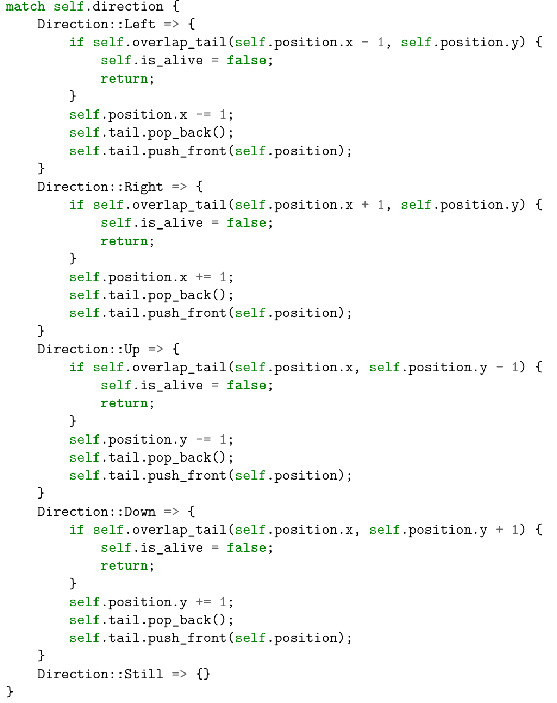
\includegraphics[width=5in]{3bi}
\subsection{}
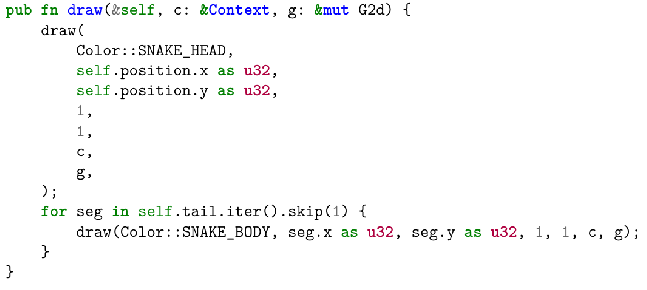
\includegraphics[width=5in]{3bii}
\subsection{}
The name of the list being used is tail.
\subsection{}
The data contained in the list represents the coordinates of the snake’s tail.
\subsection{}
The list helps manage the complexity of the code by allowing me to easily print/draw the snake’s tail on the screen. If I did not use the list there would be no way for me to accomplish this. I would have to use a list that can change its size depending on the size of the screen and the size of the snake’s tail. If the player increases the size of their screen allowing for the snake to grow longer then the list would also have to grow. The list allows for the code to still function even after changes in the game. This would be impossible to accomplish without the use of a list.

\section{}
\subsection{}
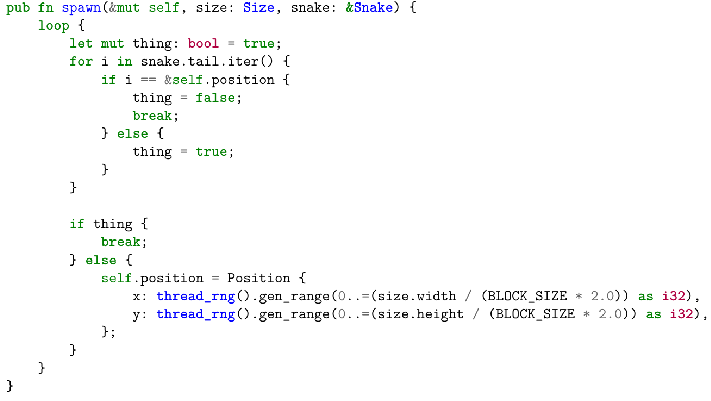
\includegraphics[width=5in]{3ci}
\subsection{}
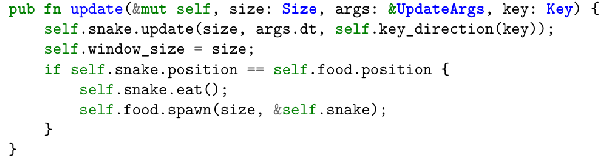
\includegraphics[width=5in]{3cii}
\subsection{}
The spawn function will generate a random coordinate that will not conflict with the location of the snake and its tail in which the food will be spawned to. This function contributes to the overall functionality of the program by allowing food to be spawned in a location that doesn’t kill the snake.
\subsection{}
The spawn function takes in 3 parameters: the food structure, the size of the window that the snake game is played in, and the snake structure. The spawn function then loops while the coordinate of the food is the same coordinate as any part of the snake’s body. Inside the loop the food’s data element ‘position’ will get updated by generating a random integer for the x and a random integer for the y part of the coordinate. The range for the random number for the x is inclusive and is from 0 to the width of the screen divided by the product of the size of the snake’s head times two. The range for the random number for the y is also inclusive and is from 0 to the height of the screen divided by the product of the size of the snake’s head times two.

\section{}
\subsection{}
The first call to the function occurs when the program is first ran, it takes in the size of the screen and the snake. This function gets ran and it generates a random coordinate that the food will be spawned to. Later through out the code whenever the player eats the food the function’s input is changed since the snake changes. The new output is another random coordinate for which the food will be spawned to, but the number of possible coordinates gets lessened by one since the snake is longer now (longer by 1 coordinate). Another possible difference in the function getting called again is if the size of the game is changed (enlarged or shrieked) the number of possible coordinate locations gets changed respectably. 
\subsection{}
The condition that is tested in the first call is if the random coordinate of the food is valid and even though the condition that is being tested in the second call is the same achieving this is different since the code will have a different output. The conditions that are tested behind this one are the if the food location is out of bounds and the other condition that is being tested is if the food is in conflict with the current location of the snake (meaning if the food is spawned on the snake).
\subsection{}
The result of the first call is a random coordinate that fits into the default parameters of the snake and screen size while the result of the second call is a new random coordinate that fits into the new parameters of the snake (the new length of the snake and the new location of the snake and its body) as well as the new parameter of the screen size. The result of the second call varies from user to user since it is completely random.

\end{document}
